Below are probability questions that I've collected. Their answers appear in the following subsection.

\subsection{List of Problems}

\begin{enumerate}
\item[1.1] What is the random variable and associated pdf and cdf of the following experiment - ``toss a coin until a head appears". Also prove that the cdf is a true cdf.

\item[1.2] Say we have a standard normal distribution that we take draws from $X_1, X_2, ...$ until we draw a value that is greater than some value $p$, in which case we stop sampling. What is the expected value of the draws?

\item[1.3] Find the probability that two points on a unit line have a distance less than 0.5. What is the probability that two random points on the border of a unit square is less than 0.5?

\item[1.4] Given the joint distribution $f(x,y) = e^{-y}$ with support $0<x<y< \infty$ find the marginal distribution of $X$, the marginal distribution of $Y$ and $P(X+Y<1)$.

\item[1.5] What is the distribution of the sum of two independent Poisson random variables, $X$ and $Y$?

\item[1.6] If $X \sim N(\mu_1, \sigma_1)$ and $Y \sim N(\mu_2, \sigma_2)$ are independent what is $Z=X+Y$ distributed as?

\item[1.7] The birthday problem - what is the probability in a room full of $n$ people that there is at least one pair that share the same birthday?

\item[1.8] A probability of success in a trial is given by $p$. For two trials, what is the probability I get two successes, given that at least one of them is a success. 

\item[1.9]
You will flip 8 fair coins in total and you've already flipped 4 of them. 3 of them have come up with tails. What is the expected number of tails by the time you've flipped all of them?

\item[1.10]
Kenzie has a 6 sided die with values 3,3,3,3,6,6 and Matt has a die with values 2,2,2,5,5,5. If they each roll the die at the same time and winner is the one with the highest number, who will win the most games in the long term?

\item[1.11]
If I get heads I put a red ball in a bag. If I get tails I put a blue ball in a bag. I do this two times so I have two balls in a bag. I then pick a ball out randomly and get a red ball. I put it back. What is the probability I chose a blue ball the second time?

\item[1.12]
Say we have 10 doors with a car behind one door. You choose one door and the game show host opens 8 other random doors. What is the probability that the car is behind the door he didn't open?

\item[1.13]
What is the probability of choosing four of a kind from a 52 card deck? (4 spades, 4 hearts, etc.). What is the probability of choosing one of each kind?

\item[1.14]
Bobo the amoeba can have zero children (with .25 prob), one child (.25), or two children (.5). What is the probability that his lineage dies out?

\item[1.15]
Imagine I have two scenarios - one where the probability of pushing a button once gives me an electrical shock with probability 0.9 and the other one where the button gives me a shock with probability 0.1 but I push it 10 times. Which scenario is better for me?

\item[1.16]
What is the probability of getting at least an 80 percent on a true false test with 20 questions if we just randomly guess?

\item[1.17]
My telephone rings 12 times each week, the calls are randomly distributed across the 7 days. What is the probability I get 4 calls one day, 2 calls on each of two days and 1 call on each remaining day?

\item[1.18]
A textbook has $n$ typos randomly scattered across $n$ pages. If we pick a random page what is the probability there are no typos on it?

\item[1.19]
In a group of $n$ people, what is the expected number of distinct birthdays (month and day)? What is the expected number of birthday matches?

\item[1.20]
There are n people at a party, each with hat. At the end of the party, they each leave with a random hat. What is the expected number of people who leave with the right hat?

\item[1.21]
In any 15-minute interval, there is a 20\% probability that you will see at least one shooting star. What is the probability that you see at least one shooting star in the period of an hour?

\item[1.22]
How can you generate a random number between 1 and 7 using a normal die?

\item[1.23]
If someone gives you a unfair coin how do you get a fair outcome from it?

\item[1.24]
You have a group of couple that decide to have children until they have their first girl, after which they stop having children. What is the expected number of children each couple will have?

\item[1.25]
How many ways can you split 12 people into 3 teams of 4?

\item[1.26]

We have a hash function that maps 10 object to elements 1-10 (inclusive), with equal probability. What is the probability of a hash collision? What is the expected number of hash collisions? What is the expected number of hashes that are unused?

\item[1.27]
You call 2 Ubers and 3 Lyfts where the time it takes for them to show up is iid. What is the probability that the first 3 that show up are Lyfts? What about for Uber?

\item[1.28]

A lazy high school senior types up n applications to colleges but randomly puts them in n envelopes addressed to each college. Whats the expected number of colleges that will get the correct applications?

\item[1.29]

What’s the expected number of coin flips until you get two heads in a row? What’s the expected number of coin flips until you get two tails in a row?

\item[1.30]

Let’s say we play a game where I keep flipping a coin until I get heads. If the first time I get heads is on the nth coin, then I pay you 2n-1 dollars. How much would you pay me to play this game?

\item[1.31]
You have a 0.1\% chance of picking up a coin with both heads, and a 99.9\% chance that you pick up a fair coin. You flip your coin and it comes up heads 10 times. What’s the chance that you picked up the fair coin, given the information that you observed?

\item[1.32]

A certain couple tells you that they have two children, at least one of which is a girl. What is the probability that they have two girls? What if I say that the oldest child is a girl what is the probability both are girls then?

\item[1.33]
I write a program should print out all the numbers from 1 to 300, but prints out Fizz instead if the number is divisible by 3, Buzz instead if the number is divisible by 5, and FizzBuzz if the number is divisible by 3 and 5. What is the total number of numbers that is either Fizzed, Buzzed, or FizzBuzzed?

\item[1.34]
This problem is commonly known as the coupon collector problem. There are n coupon types. At each draw, you get a uniformly random coupon type. What is the expected number of coupons needed until you have a complete set?


\end{enumerate}

\subsection{Answers}

\begin{enumerate}

\item[1.1] What is the random variable and associated pdf and cdf of the following experiment - ``toss a coin until a head appears". Also prove that the cdf is a true cdf.

First of all we recognize that this is a geometric distribution which counts the number of failures until the first success. The geometric pmf is given by:

\begin{equation}
q^{x}p
\end{equation}

\noindent where $q$ is the probability of failure, $p$ is the probability of success, and $x$ is the number of failures. The support is on all nonnegative integers. 

We note that the pmf gives the distribution of number of failures whereas we want to include the time the coin actually appears heads. Therefore we want $x+1$. This requires a transformation where $g(X) = X + 1$.

Using equation \ref{eq:pmf_transform} we have for $Y=g(X)$ and $g^{-1}(Y) = Y - 1$:

\begin{equation}
f_Y(y) = \sum_{x \in g^{-1}(y)} P(X = x) = \sum_{x \in g^{-1}(y)} q^{x}p = q^{y-1} p
\end{equation}
\noindent The last step occurs because $g$ is a one-to-one function and the only $x$ that maps to our $y$ is $y-1$. 

Now that we have our pmf, we want to find the cdf. This is done by doing the following

\begin{equation}
F_Y(y) = P(Y \leq y ) = \sum_{i=1}^{y} (1-p)^{i-1}p  = p \left [ \frac{1 - (1-p)^y}{1 - (1-p)} \right ] = 1 - (1-p)^y
\end{equation}
\noindent by the geometric series.

To prove this is a cdf we show that as $y$ goes to $-\infty$ we get 0 (which is true because $F_Y(y)$ is defined to be 0 for $y<0$, as it goes to $\infty$ we get 1 (which is true because $1-p$ is a number less than 1 and raised to infinity goes to 0), it is monotonically increasing, and lastly we show it is right continuous by $F_Y(y+\epsilon) = F_Y(y)$ as $\epsilon$ goes to 0. 



\item[1.2] Say we have a standard normal distribution that we take draws from $X_1, X_2, ...$ until we draw a value that is greater than some value $p$, in which case we stop sampling. What is the expected value of the draws?

The first step is to write down what we want. The way to think of this is that we want to know the expected value of $X$ (where $X$ is a normal random variable), but with the condition that $X<p$. This can be written as $ E[X|X<p]$. Using the standard normal distribution we have:


\begin{align*}
E[X|X<p] &= \int_{-\infty}^{\infty} x f_X(x|X<p) dx \hspace{2em}  \text{(by definition of expectation)}\\ 
&=  \int_{-\infty}^{\infty} x \frac{f_X(x, X<p)}{P(X<p)} dx  \hspace{2em} \text{(by definition of conditional probability)} \\
&= \frac{1}{P(X<p)} \int_{-\infty}^{p} x \frac{1}{\sqrt{2\pi}}e^{\frac{-x^2}{2}} dx \hspace{2em} \text{(limit integral bounds to match conditional prob.)} \\
&= \frac{1}{P(X<p)\sqrt{2\pi}} \int_{-\infty}^{p} x e^{\frac{-x^2}{2}} dx
\end{align*}

\noindent The quantity $P(X<p)$ is given by the cdf of the standard normal distribution. The integral, using u-substitution, is found to be:

\begin{equation}
\begin{split}
\int_{-\infty}^{p} x e^{\frac{-x^2}{2}} dx  &= \int_{-\infty}^{\frac{-p^2}{2}} - e^{u} du \\
&= -e^{\frac{-p^2}{2}} + e^{-\infty} \\
&= -e^{\frac{-p^2}{2}}
\end{split}
\end{equation}
\noindent where $u=\frac{-x^2}{2}$.

All together we have $\frac{-e^{\frac{-p^2}{2}}}{P(X<p)\sqrt{2\pi}}$. If $p=1$ for example then we have 

\begin{equation}
\frac{-e^{\frac{-1}{2}}}{P(X<1)\sqrt{2\pi}} \approx \frac{-e^{\frac{-1}{2}}}{0.84*\sqrt{2\pi}} \approx -0.288
\end{equation}


One question I had is if there is a difference between taking the expectation of a sequence from the distribution and stopping once we have a value that is greater than $p$ vs. taking the expectation of a set sample with variables that are greater than $p$ thrown out. 

From a simulation perspective there is no difference if we think of the set sample as a bunch of sequences tied together, broken up by the values greater than $p$. In this light, the sequences are essentially defined by the realizations that are greater than $p$. So even though thinking about this process from a sequence point of view, I feel it is safe to conclude that we are just taking the normal random sample process approach, looking for the expectation of $X$ conditioned on the event that $X<p$. 

The code for this simulation is given below:

\begin{lstlisting}[language=Python]
from scipy.stats import norm
import numpy as np

mean_rvs = []
N = 10000
p = 1
for i in range(N):
    rvs = []
    less = True
    while less:
        rv = norm.rvs(size=1) # sample one normal, standardized random variable
        if rv < p: # if draw is less than p, add to sequence
            rvs.append(rv[0])
        else: # if draw is greater than p, stop sequence
            less=False
    if len(rvs)!=0: # take mean of sequence, as long as there is as least one random variable in sequence
        mean_rvs.append(np.mean(rvs))
\end{lstlisting}
\noindent where the mean of ``mean\_rvs'' is around -0.288.


\item[1.3] Find the probability that two points on a unit line have a distance less than 0.5. What is the probability that two random points on the border of a unit square is less than 0.5?


\begin{equation}
\begin{split}
P(|Y-X| < 0.5) &= P(-0.5 < Y-X < 0.5) \\
&= P(Y-X < 0.5) - P(Y-X < -0.5) \\
&= P(Y < X + 0.5) - P(Y < X - 0.5)
\end{split}
\end{equation}

We can think of $Y, X$ having a joint uniform distribution on the unit square. This gives us every possible combination of these two variables. If we think of it in this context and relate the two variables together then we can deal with the probability terms above. 

The first part of the last expression above is going to be the area (since this is the uniform distribution) below the line $Y = X + 0.5$ on the unit square. This ends up being $\frac{7}{8}$. The second part will be the area below the line $Y < X - 0.5$ which ends up being $\frac{1}{8}$. Therefore we have a difference of $\frac{6}{8}$ or 0.75. 

The second part to this question requires knowing the probability of two points in general on the unit square having a distance less than 0.5. To answer this assume that one point falls on the bottom of the box and the other on the right of the box. We can then use the pythagorean theorem to get:

\begin{equation}
\begin{split}
P(\sqrt{(1-X)^2 + Y^2} < 0.5) &= P((X-1)^2 + Y^2 < 0.25) 
\end{split}
\end{equation}
\noindent We can recognize this quantity within the probability as the equation of a circle where the center is at $(1,0)$. If we draw this on the unit square and find the area of the intersection we see that the probability is $\frac{\pi}{16}$ (we need to just find the area since it is distributed uniformly, if it were another distribution we would need to actually do an integral.) 

We find that no matter which two adjacent sides the points are on we will still have a probability of $\frac{\pi}{16}$. 

At this point we want to use the law of total probability to split up the event $A$ where $A$ equal ``the probability two points on a unit square are less than 0.5'':

\begin{equation}
\begin{split}
P(A) &= 4*P(A|B)P(B) + 8*P(A|C)P(C)
\end{split}
\end{equation}
\noindent I've obviously skipped some steps here but the ideas is this: if we choose random two points on the unit square then there is a $\frac{1}{16}$ chance they appear on the same side which is what $P(B)$ is representing. We already know $P(A|B)$ is 0.75 from the previous discussion and we multiply it by 4 since there are 4 sides. One thing I was confused on is why we don't multiply it by 8 since the points could be reversed but if we think of assigning two points to the four different sides and every possible combination this would be double counting a combination.

The second part of the equation shows the probability of two points being on adjacent sides $P(C)$ which is also $\frac{1}{16}$ and we know that $P(A|C)$ is $\frac{\pi}{16}$. We multiply by 8 since there are 4 possibilities of adjacent sides and where each point could be switched leading to 8 cases. 

I've omitted the last case where the points are on opposite sides since these distances will be larger than 1 so the probability of it being less than 0.5 is 0.

Adding this all up we get around 0.28567.

I verify this in simulation code below:

\begin{lstlisting}[language=Python]
sim_size = 200000
distances = np.zeros(sim_size)
for i in range(sim_size):
    x = np.random.uniform(0,4.0)
    y = np.random.uniform(0,4.0)

    if x <= 1.0:
        point_x = (x,0.)
    elif x > 1.0 and x<=2.0:
        point_x = (1.,x-1)
    elif x > 2.0 and x <= 3.0:
        point_x = (1-(x-2), 1.)
    else:
        point_x = (0, 1-(x-3))
        
    if y <= 1.0:
        point_y = (y,0.)
    elif y > 1.0 and y<=2.0:
        point_y = (1.,y-1)
    elif y > 2.0 and y <= 3.0:
        point_y = (1-(y-2), 1.)
    else:
        point_y = (0, 1-(y-3))
    
    distances[i] = la.norm(np.array(point_x) - np.array(point_y))
    
sum(distances <.5)/(sim_size*1.0)
\end{lstlisting}


\item[1.4]
Given the joint distribution $f(x,y) = e^{-y}$ with support $0<x<y< \infty$ find the marginal distribution of $X$, the marginal distribution of $Y$ and $P(X+Y<1)$.

The best approach to these problems is to visualize the support as in Figure \ref{fig:support}. To find $P(X+Y<1)$ we can rearrange the equation to equal $P(Y<1-X)$. The way to think of this quantity is the probability of an event $Y<1-X$ which is the integral of the pdf over every possible $Y,X$ in the support and that satisfies the above equation. This limits our integral to the support found in Figure \ref{fig:support2}. 

 \begin{figure}[t] \label{fig:support}
\caption{Support for joint probability function $f(x,y) = e^{-y}.$}
\centering
 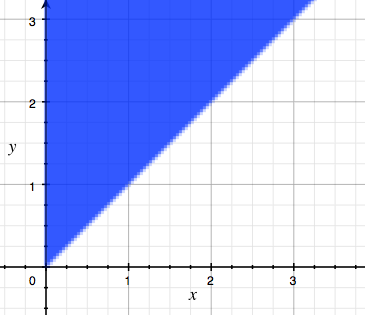
\includegraphics[scale=.7]{support.png}
 \end{figure}
 
  \begin{figure}[t] \label{fig:support2}
\caption{Area to integrate over}
\centering
 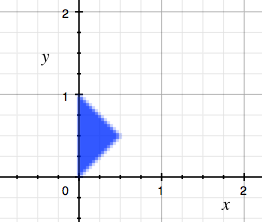
\includegraphics[scale=.7]{support2.png}
 \end{figure}
 
 
 Our integral therefore is:
 
 \begin{equation}
 \begin{split}
 \int_0^{0.5}{\int_x^{1-x}{e^{-y}dy}dx} &= \int_0^{0.5}{-e^{-1+x} + e^{-x}dx} \\
& =  -e^{-1+0.5} - e^{-0.5} + e^{-1} + 1 \\
& \approx 0.1548181217
 \end{split}
 \end{equation}
 
 To find the marginal of $X$ we take the integral over all $Y$:
 
 \begin{equation}
 \int_x^{\infty}{e^{-y}dy}
 \end{equation}
 
 \noindent To find the marginal of $Y$ we take the integral over all $X$:
 
 \begin{equation}
 \int_0^{y}{e^{-y}dx}.
 \end{equation}
 
 
\item[1.5] \label{item:sum_possion}

What is the distribution of the sum of two independent Poisson random variables, $X$ and $Y$?

If we take the bivariate transformation approach we want one variable to be the sum of $X$ and $Y$ so that we can marginalize the other variable out to get this distribution. Therefore we let $U=X+Y$ and $V=Y$. The support of $X$ and $Y$ are the non-negative integers so the support of $V$ will be the same and the support of $U$ will be $v, v+1, ...$ since $u=x+v$.

When determining which values $(x,y)$ we need to sum over for each $(u,v)$ we ask for any $(u,v)$ pair what are the $(x,y)$ values that give me that pair or in other words what $(x,y)$ values solve both equations? The answer is $x=u-v$ and $y=v$. We can then plug this into the bivariate transformation formula where we sum over one tuple of values $(u-v, v)$ (sub this in for $X$ and $Y$ in the pdf of $(X,Y)$.

The next step is to sum over all $V$ to get the marginal pmf of $U$ which will give us the distribution of $X+Y$. It is important to remember when doing this that we take a close look of the support of this joint pmf. We'll notice that since $U$ is dependent on $V$ that the support is to the side of the line $u=v$. Therefore when summing over $V$ we go from $v=0$ to $u$.

\item[1.6]

If $X \sim N(\mu_1, \sigma_1)$ and $Y \sim N(\mu_2, \sigma_2)$ are independent what is $Z=X+Y$ distributed as?

There are a couple of approaches here. One approach is to use the MGF of each variable. We know that the MGF of a sum of independent random variables is the product of the separate MGF's. In this case we find that the product of the separate MGFs yields a MGF in the same form as the normal MGF and we can then take out the necessary parameters to conclude that the distribution of  $Z$ is $N(\mu_1+\mu_2, \sigma_1+\sigma_2)$.

The other option is to use the Bivariate transformation where we choose $U=X+Y$ and $V=X$, or better yet we can just use the convolution formula which is just the Bivariate transformation anyways.

The last option is to look at $F_Z(x) = P(Z<z) = P(X+Y<z)$ and integrate over the area of the joint distribution $f_{X,Y}(x,y)$. 

A better example (to avoid having to integrate everything) for these last two approaches is when we have two independent uniform random variables. Using the convolution we have:

\begin{equation}
f_Z(z) = \int f_X(w)f_Y(z-w)dw
\end{equation}

When we take this approach we have to be careful about the bounds of integration. We know that since $W=X$ that $0<W<1$. When looking at the bounds of $Z$ we know that $Z=W+Y$ and when $W=0$, $0<Z<1$ and when $W=1$, $1<Z<2$. A good illustration of this comes from \href{https://math.stackexchange.com/questions/357672/density-of-sum-of-two-uniform-random-variables-0-1}{this} Stack Overflow question and is shown in Figure \ref{fig:uniform_support}.

\begin{figure}[t] \label{fig:uniform_support}
\caption{Joint uniform support}
\centering
 
\includegraphics[scale=.7]{uniform_support.png}
 \end{figure}

Because of this when we integrate our $W$ we consider two cases - when $Z$ is greater than 1 and less than 1. When less than 1 we integrate out $W$ using the bounds 0 to $z$ and find that the resulting pdf is $z$. When $z$ is between 1 and 2 we use the bounds $z-1$ to 1 and find the the pdf is $2-z$. 

If we take the other approach $P(X+Y<z)$ and look at integrating over the joint distribution $X,Y$ we again need to consider the two cases. For example, when $z<1$ our bounds for integrating over $X$ will be from 0 to the line $Y=z - X$ (or $z-y$ when integrating) and the bounds for $Y$ will be from 0 to $z$. These bounds change when $z>1$ so we have to calculate a separate integral.

This whole exercise illustrated the importance of understanding the support of a joint distribution in order to calculate integrals correctly. If we hadn't figured out the support then we wouldn't have realized the need to break up into cases.

\item[1.7] The birthday problem - what is the probability in a room full of $n$ people that there is at least one pair that share the same birthday?

The first step to this problem is to recognize the ``at least" one pair verbage. This should be a signal to change the probability we are trying to find to the probability that there are no matches and then do 1 minus that quantity. 

We go straight to the naive definition of probability and find all possible combinations in the denominator and all combinations for the event in the numerator. For the denominator we go back to our 2x2 table and ask what is $n$ and $k$ and is this w/wo replacement and does order matter/not matter. In this case $n$ is referring to the number of days in the year and $k$ is referring to the number of people. When considering all possibilities then we are sampling with replacement and we say that order does matter since people are distinguishable (July 1st for person 1 and July 1st for person 2 are two different possibilities). 

On the numerator we have the same thing but this time we sample without replacement because we are counting how many ways can we get birthdays where no two people share the same bday. Once a birthday is picked it can't be picked again.

This leaves us with
\begin{equation}
P(A) = 1 - P(A^{c}) = 1 - \frac{\frac{365!}{(365 - k)!}}{365^k}
\end{equation}

\item[1.8] A probability of success in a trial is given by $p$. For two trials, what is the probability I get two successes, given that at least one of them is a success. 

My initial reaction to this question is to list out all of the possibilities (our sample space), $S$ for success and $F$ for failure. We would therefore have $S,S$, $S,F$, $F,S$, $F,F$. Given that at least one of the trials is a success then we are down to three options and only one of those options both trials were a success. Therefore the probability would be $\frac{1}{3}$.

The problem with this approach however is that I am assuming all possibilities are equally likely, which is only the case when $p=\frac{1}{2}$. Instead of going directly to the naive definition of probability it would have been better to use the definition of conditional probability which can be written as:

\begin{equation}
P(A|B) = \frac{P(A\cap B)}{P(B)}
\end{equation}
\noindent where $B$ is ``at least one success'' and $A$ is ``both success''. The numerator is $p^2$ since the intersection of at least one success and both success is really both success. The denominator is a little more tricky but because we see ``at least one'' we can change it to $1-P(B^c)$ where $B^c$ is ``no success''. This would therefore give us:

\begin{equation}
\begin{split}
\frac{p^2}{1 - (1-p)^2} &= \frac{p^2}{1 - (1-2p+p^2)} \\
&= \frac{p^2}{2p-p^2} \\
&=\frac{p}{2-p}
\end{split}
\end{equation}
\noindent Plugging in .5 for $p$ gives us $\frac{1}{3}$ as expected. 


\item[1.9]
You will flip 8 fair coins in total and you've already flipped 4 of them. 3 of them have come up with tails. What is the expected number of tails by the time you've flipped all of them?

This one is tricky for me and I fell right into whats called the ``gamblers fallacy'', the idea that because we've seen a bunch of tails means we should see a bunch of heads for the next four. This is confusing two concepts I think - the long term behavior of the coins and independence of each flip. If you think about it, it doesn't matter at all what we've got in the past. Each flip is independent. So therefore the expected number of tails in this scenario is 5 since we expect 2 more tails in the remaining 4.

\item[1.10]
Kenzie has a 6 sided die with values 3,3,3,3,6,6 and Matt has a die with values 2,2,2,5,5,5. If they each roll the die at the same time and winner is the one with the highest number, who will win the most games in the long term?

Intuitively looking at these numbers I would say that Kenzie will win the most times. I initially tried to solve this by looking at the expected values which end up being the same. The reason this is the wrong approach is because I don't care what the average value is for each person - I care what they role on a particular time and how it \emph{compares} to the other person.

The first step to this is determining what our sample space is. If we look at every possible dice combination (36) possibilities we can then reason that half the time (when we are matched up with 2) Kenzie will win (18 times). For the other 18 scenarios Kenzie will win 6 times. Therefore 24/36 = 2/3

\item[1.11]
If I get heads I put a red ball in a bag. If I get tails I put a blue ball in a bag. I do this two times so I have two balls in a bag. I then pick a ball out randomly and get a red ball. I put it back. What is the probability I chose a blue ball the second time?

The key information to pick out here is that once we know the first ball is red then it narrows down the possibilities. I was frustrated with this problem because I didn't know how to break down the conditional probability using Bayes rule or law of total probability, etc. Using the law of total probability is weird because you get an empty set in one of the conditionals. Using Bayes doesn't seem the approach either because how do you have a conditional on something that happens in the future (picking the blue ball?).

I think the best approach here is to first do a conditional and then law of total probability on denominator and numerator. The reason it makes sense to do the law of total probability is because there is this initial probability breakdown at the beginning (the process we put balls into the bag).

\begin{equation}
\begin{split}
P(B|A)  & = \frac{P(B \cap A)}{P(A)} \\
&=  \frac{P(B \cap A|RR)P(RR) + P(B \cap A|RB)P(RB) + P(B \cap A|BR)P(BR) + P(B \cap A|BB)P(BB)}{P(A|RR)P(RR) + P(A|RB)P(RB) + P(A|BR)P(BR) + P(A|BB)P(BB) } \\
&= \frac{0 + \frac{1}{16} + \frac{1}{16} + 0}{\frac{1}{4} + \frac{1}{8} + \frac{1}{8}} \\
&= \frac{1}{4}
\end{split}
\end{equation}

If we change the wording to ``I look in the bag and say there is at least one red ball in there" and I pull one red ball out the problem changes. I'm not sure how to translate that into probability formulas above. I guess reasoning that when you pull out a red ball on purpose that isn't an event we attach probability to - its just something you did. You will always be left then with with a blue ball, a blue ball, or a red ball in the bag, therefore $\frac{2}{3}$ is the answer. 

\item[1.12]
Say we have 10 doors with a car behind one door. You choose one door and the game show host opens 8 other random doors. What is the probability that the car is behind the door he didn't open?

With these its best to simplify and choose a door that we pick, say door 1. You can then calculate the probability and then if we say instead, that we chose door 2, the probability will be the same since the doors are indistinguishable.

Bayes rule all the way baby! So going with door 1 we want to know what is the probability the car is behind this door \emph{given} that the host opens a specific 8 doors.

Let $A$ be ``door 1 has car", $B$ be ``8 doors opened'', and $C$ be ``door 2 has car''.

\begin{equation}
P(A | B) = \frac{P(B|A)P(A) }{P(B)}
\end{equation}

The first probability is going to be $\frac{1}{9}$ since there are 9 ways to open up 8 doors from 9 available doors (since the car is really behind door 1). The second probability is just $\frac{1}{10}$ the probability to begin with.

We then use the law of total probability on the bottom. So for example $P(B | C) P(C)$ is $\frac{1}{9}\frac{1}{10}$ multiplied by 10. Therefore overall we have $\frac{1}{10}$. Therefore switching to the available door is a $\frac{9}{10}$ probability. 

The key is to look at $P(B | C) P(C)$ by itself, ignoring that we chose door 1.

\item[1.13]
What is the probability of choosing four of a kind from a 52 card deck? (4 spades, 4 hearts, etc.). What is the probability of choosing one of each kind?

So we first realize that each outcome is equally likely so we can use the naive definition of probability. Since order doesn't matter and we are doing this without replacement then on the denominator we have $52 \choose 4$. For the denominator then we have for hearts for example $13 \choose 4$. This gives us all the ways we can choose 4 cards from the heart group. We multiply this by 4 on the top (since we are adding the number of possibilities to the other groups.

The key to thinking about all of this is that when we lay out our denominator we can think of every possible draw of 4 cards. Some of those draws with all be hearts. We have to ask ``well how many of those draws will be hearts'' thus $13 \choose 4$.

For 4 of each kind we use the same denominator but we recognize that only 13 times will there be 4 of each kind (because there are 13 numbers).

\item[1.14]
Bobo the amoeba can have zero children (with .25 prob), one child (.25), or two children (.5). What is the probability that his lineage dies out?

This is a perfect application of the law of total probability. We want to know $P(A)$ where $A$ is the event that Bobo's lineage dies out. We use total probability to say:

\begin{equation}
P(A) = P(A|B)P(B) + P(A|C)P(C) + P(A|D)P(D)
\end{equation} 
\noindent where $B,C,D$ are probability of 0 child, 1 child and 2 children. Filling out the values we then have:


\begin{equation}
P(A) = (1).25 + P(A)*0.25 + P(A)^2 * 0.5
\end{equation} 

We can substitute in $P(A)$ because each member of his posterity has the same probability of their linear dying out. Solving for $P(A)$ we get 0.5. Note that solving this was somewhat extensive including using complete the square method. 

\item[1.15]
Imagine I have two scenarios - one where the probability of pushing a button once gives me an electrical shock with probability 0.9 and the other one where the button gives me a shock with probability 0.1 but I push it 10 times. Which scenario is better for me?

First we define the event $A$ for scenario 2 to be ``pushing a button 10 times and getting shocked at least once''. Recognizing the ``at least once'' language we take the complement of this and look to find $P(A^{c})$ or the probability of pushing a button 10 times and not getting shocked at all. This can be thought of as $0.9^{10}$ which is around 0.34. Subtracting this from 1 we get around 0.66 which is much less than 0.9. 

\item[1.16]
What is the probability of getting at least an 80 percent on a true false test with 20 questions if we just randomly guess?

Define the event $A$ as getting at least 80 percent which would be getting 16, 17, 18, 19, or all 20 right. We want $P(A)$. Since we are randomly guessing all possible outcomes are equally likely. Therefore we use the naive definition of probability. 

The first question we ask is what do we put on the denominator. We want to put all possible outcomes so the correct number is $2^{20}$. This is because we have a with replacement (drawing from the possibilities true/false) and order matters scenario. 

For the numerator we think of finding all possible ways of getting 16 questions correct which would be 20 choose 16. This has always been a source of confusion for me because on the bottom we are in a with replacement, order matters scenario but on top we are in a without replacement, order does not matter scenario. Seems like they should be the same. The reason there is a difference however is because in the top our outcomes we are sampling from are the questions themselves whereas in the denominator the outcomes are either true or false. In the numerator we are selecting which question numbers are going to be true and all the ways of doing that. 

Since we said at least 80 percent then we need to also include all of the ways of getting 17 questions correct, 18, etc. 
 
\item[1.17]
My telephone rings 12 times each week, the calls are randomly distributed across the 7 days. What is the probability I get 4 calls one day, 2 calls on each of two days and 1 call on each remaining day?

This one puzzled me for the longest time but there are some subtleties to be aware of. As usual we define our event A to be 4 calls one day, 2 calls on each of 2 days and 1 call on the remaining days. We want to find $P(A)$. 

To do this we first recognize that each outcome is equally likely so we can use the naive definition of probability. The first step is then to determine what is on the denominator or every possible outcome. In this case we want $7^{12}$ which are all the possibilities of assigning days of the week to the 12 calls. 

The numerator is where it gets tricky. To best think of this imagine in your mind what the denominator is counting, or what each possibility is representing. In this case we can imagine 12 phone call ``slots'' with a day assigned to them. So using this image we need to create the scenario of event A.

We first think of choosing 4 random phone call slots from 12 possibilities. Since order doesn't matter and we are doing this without replacement then we have 12 choose 4. That gives us 495 different ways of choosing 4 phone call slots. We now need to assign days to these slots and since all 4 phone calls fall on the same day then we have 7 choose 1 or in other words 7 different possibilities. so 7*495=3465 different ways of assigning 4 slots to one of 7 different days. 

But wait theres more! We've only picked a random 4 slots. What about the remaining other 8 slots? We want to pick two of those slots to fall on a given day and then after that another two to follow on a given day. This is the tricky part because my first instinct was to do 8 choose 2 (to select 2 random slots from the 8 remaining ones) and then do 6 choose 1 (to select a day to assign to the slots from the six remaining days). Then I would do 6 choose 2 followed by 5 choose 1. 

This is the wrong approach however. The correct approach is 8 choose 2 followed by 6 choose 2 and then for the days followed by another 6 choose 2. The reason we take this approach is because the first one double counts possibilities. We might select slots 1 and 2 for example and assign it to day 1 followed by selecting slots 3 and 4 and assigning it to day 2. In my first scenario we are not only counting the correct possibilities (slots 1 and 2 assigned to 1, slots 3 and 4 assigned to 2,  slots 3 and 4 assigned to 1, slots 1 and 2 assigned to 2) but counting then twice because we are switching slots AND days around. This is a subtle point that was not intuitive to me. 

The remainder is for assigning the slots 4 choose 1, 3 choose 1, 2 choose 1, 1 choose 1, and finally 4 choose 4 when selecting the days. All of these are multiplied together. 

\item[1.18]
A textbook has $n$ typos randomly scattered across $n$ pages. If we pick a random page what is the probability there are no typos on it?

We want $P(A)$ where $A$ is the event that there are no typos on a randomly chosen page. We can logic through this by realizing that the errors will be randomly distributed meaning for a given page there is a $\frac{1}{n}$ chance that we have a specific typo. This implies then that the probability of not having that specific typo is $(1 - \frac{1}{n})$. To not have any of the typos we then have $(1- \frac{1}{n})^n$.

\item[1.19]
In a group of $n$ people, what is the expected number of distinct birthdays (month and day)? What is the expected number of birthday matches?

The first question is asking for an expectation. Since we are counting here a natural step would be to use linearity and expectation.

We think of a sum of indicator random variables $I_i$ where the sum is the number of distinct birthdays and each $I_i$ is an indicator whether or not a given day in the year is in the group. We then are concerned with the probability that we have this birthday amongst $n$ people.

To get this probability we go to the definition of naive probability and look at the probability it is not a distinct birthday. The denominator will be $365^{n}$ because thats the number of ways of getting $n$ birthdays and the numerator will be $364^n$ because thats the number of ways of choosing $n$ birthdays without the current day. This means the probability it is a distinct birthday will be $1 - (\frac{364}{365})^n$. 

Taking the expectation of this sum we get $365*(1 - (\frac{364}{365})^n)$.

The second question we take the same approach but this time $I_i$ will represent person $a$ and person $b$ have the same birthday. The probability of them not having a shared birthday will be $365^2$ in the denominator and $365*364$ in the numerator.

In total we will have ${n \choose 2 } (1 - \frac{364}{365})$.


\item[1.20]
There are n people at a party, each with hat. At the end of the party, they each leave with a random hat. What is the expected number of people who leave with the right hat?

Again lets divide this random variable into indicator random variables where each $I_i$ is if a person left with his/her hat. The probability of this happening is $\frac{1}{n}$. When we take the expected value of these indicators we 1. 

\item[1.21]
In any 15-minute interval, there is a 20\% probability that you will see at least one shooting star. What is the probability that you see at least one shooting star in the period of an hour?


The first step is to realize that this is a Poisson random variable. We recognize it as such because we are dealing with counts (number of shooting stars) that have many ways of occurring but don't happen often. 

The next step is to recognize this as a poisson process. We can recognize it as such if we make the following assumptions: for any time interval the count is modeled by a poisson distribution, and each time interval is independent of the other.

One time interval is 15 min. We want to know over 4 time intervals (an hour) what the count is. Therefore we can use the properties of the poisson process to write $Pois(4\lambda)$. We want to know the probability of at least one shooting start so for now lets do the complement of zero shooting stars:

\begin{equation}
\frac{\lambda^{0} e^{-4\lambda}}{0!}
\end{equation}

We want to know what $\lambda$ which we can find using one time interval and the complement again:

\begin{equation}
e^{-\lambda} = .8
\end{equation}

Therefore $\lambda$ is equal to $-ln(0.8)$. Plugging this into our previous equation and taking the complement we get:

\begin{equation}
1 - (0.8)^4
\end{equation}

\item[1.22]
How can you generate a random number between 1 and 7 using a normal die?

Use binary numbers. Roll the die three times. If it is 1-3 then set equal to 1 otherwise set equal to 0.

\item[1.23]
If someone gives you a unfair coin how do you get a fair outcome from it?

Flip it twice. If it comes up H,H or T,T ignore it. If it comes up H,T  then call it heads. If it comes up T,H call it tails. This is because these two quantities both have a probability of $(1-p)p$ of occurring if $p$ is the probability of a heads.


\item[1.24]
You have a group of couple that decide to have children until they have their first girl, after which they stop having children. What is the expected number of children each couple will have?

First let's define relevant terms. We see expected number of children so we know we are dealing with random variables. Let $X$ be the number of children each couple will have. We then have to ask which distribution it follows, which we can recognize as the geometric distribution transformed to count the first success. Therefore the expectation will be $\frac{1}{p}$ or since our probability of a girl 0.5 then our expectation will be 2.

\item[1.25]
How many ways can you split 12 people into 3 teams of 4?

I'm not super clear on this but I'm pretty sure if the teams are distinguishable then we would use the multinomial coefficient ${12 \choose 4, 4, 4}$. The way to understand why this is so is to first think of the number of ways we can choose one team of 4 from 12 people. We know this to be  ${12 \choose 4}$. Then we multiply that by  ${8 \choose 4}$ (for the second team) and finally  ${4\choose 4}$. Multiplying this all together gives us  ${12 \choose 4, 4, 4}$.

If the teams are indistinguishable though I wonder if we want ${12 \choose 4, 4, 4, 3}$ to account for duplicate teams. 


\item[1.26]

We have a hash function that maps 10 object to elements 1-10 (inclusive), with equal probability. What is the probability of a hash collision? What is the expected number of hash collisions? What is the expected number of hashes that are unused?

The first question is easy if you utilize the multinomial distribution. If we think of the probability of no hash collisions then we want to find the probability of the vector $(1,1,1,1,1,1,1,1,1,1)$. According the multinomial distribution this will just be:

\begin{equation}
\frac{10!}{1!1!1!1!1!1!1!1!1!1!} (\frac{1}{10})^{10}
\end{equation} 

The next question is a bit trickier. It might be easier to first think of the expected number of hashes that are unused. This is done by letting the indicator be 1 if the hash is unused and 0 if it is used. So for slot $j$ for example, the probability that it is empty is the same as saying that an object isn't assigned to it $(1-\frac{1}{k})$ for all objects $(1-\frac{1}{k})^n$ where $k$ is number of bins and $n$ is number of objects. The expectation will therefore be $n*(1-\frac{1}{k})^n$.

When wanting to figure out the expected number of collisions we treat $X$ as the number of empty hash's and therefore the number of collisions will be $n - k + X$ (since $k-X$ gives us the number of nonempty bins, and subtracting that from $n$ will give us the number of overlap or collisions. If we take the expectation of that we get $n - k + n*(1-\frac{1}{k})^n$. Subbing in $k=10$ and $n=10$ we get $10*(1 - \frac{1}{10})^{10}$. 


\item[1.27]

You call 2 Ubers and 3 Lyfts where the time it takes for them to show up is iid. What is the probability that the first 3 that show up are Lyfts? What about for Uber?

There are a couple of ways of solving this. My first thought was to use the naive definition of probability since all outcomes are equally likely. On the denominator then I would have ${5 \choose 3}$ giving us all the ways of picking from the 5 cars, 3 cars to show up first. Only one of those will be all 3 Lyfts. Therefore the probability will be $\frac{1}{10}$.

The second question will be the same because ${5 \choose 2}$ is equal to ${5 \choose 3}$.

Another way to think of this is to multiple probabilities together. So for the first question the probability that the first car shows up is a Uber is $\frac{3}{5}$ and the probability of the second car is $\frac{2}{4}$ and the third is $\frac{1}{3}$. Multiplied together gives us $\frac{1}{10}$.

\item[1.28]

A lazy high school senior types up n applications to colleges but randomly puts them in n envelopes addressed to each college. Whats the expected number of colleges that will get the correct applications?

This is the same problem as the n hats in the room. Simply think of the high school senior putting all n applications in a pile. Then let $X_1$ be an indicator for his first draw - 1 if he gets the right application to the right folder, and 0 if he doesn't. The probability of 1 is $\frac{1}{n}$ so by linearity the expected value is 1.

As a variation on this I wonder if you used the wording ``if the senior took a random envelope and a random application" the outcome would change because the probability would be $\frac{1}{n^2}$ instead of $\frac{1}{n}$.

\item[1.29]

What’s the expected number of coin flips until you get two heads in a row? What’s the expected number of coin flips until you get two tails in a row?

This one is a tricky one and one that is best solve using recursion and not playing with the traditional definition of expectation.

The first idea is to let $x$ be the expected number of flips until we get two heads in a row. Say we flip the coin one time and get a tails. We know then that our total number of flips will be $x+1$. The probability of this happening is $\frac{1}{2}$. If we flip a heads the first time and a tails the second time then we have $x+2$. The probability of this happening is $\frac{1}{4}$. If the first two flips are heads then the count is 2 with probability $\frac{1}{4}$. Our equation then becomes:

\begin{equation}
x = .5(x+1) + .25(x+2) + .25(2)
\end{equation}

Therefore  $x=6$

\item[1.30]

Let’s say we play a game where I keep flipping a coin until I get heads. If the first time I get heads is on the nth coin, then I pay you 2n-1 dollars. How much would you pay me to play this game?

This is an expected value question. We want to know what the expected payout is. Lets write this out:

$.5*(1) + .25*3 + .125*5 + ... + $

We recognize this as an arithmetico-geometric series. The numerator varies by a additive constant (2) and the denominator varies by a multiplicative constant (.5). 

We can solve this by letting $S = .5*(1) + .25*3 + .125*5 + ... + $. If we have $\frac{S}{2} = .25*(1) + .125*3 + .0625*5 + ... + $ then $S - \frac{S}{2} = .5 + .5 + .25 + 0.125 + ... + ... $. Therefore $\frac{S}{2} = .5 + .5 + .25 + 0.125 + ... + ... $, therefore $S = 1 + 1 + .5 + .25 + ... $. The first two terms sum to 2 and all other terms are the geometric series which sums to 1 so all together we have 3. This is the expected payout our friend will pay. So we would only want to pay him less than that. 
  
\item[1.31]
You have a 0.1\% chance of picking up a coin with both heads, and a 99.9\% chance that you pick up a fair coin. You flip your coin and it comes up heads 10 times. What’s the chance that you picked up the fair coin, given the information that you observed?

Bayes rule all the way!

Should be around 0.5.

\item[1.32]

A certain couple tells you that they have two children, at least one of which is a girl. What is the probability that they have two girls? What if I say that the oldest child is a girl what is the probability both are girls then?

If we assume that all possibilities are equal then we could list out the possibilities, only include the ones where there is at least one girl, and then find that $\frac{1}{3}$ will be two girls.

Perhaps the more fail safe way however to tackle this is to use conditional probability and write:

\begin{equation}
P(A|B) = \frac{P(A \cap B)}{P(B)}
\end{equation}
\noindent where $A$ is the event that there are two girls and $B$ is the event that there are at least one girl. We no that the numerator will be .25 (since $B$ is a subset of $A$ and the probability of having two girls is $0.5 * 0.5$). The denominator will be 0.75 since we have .5*.5 + .5*.5 + .5 *.5. The event is $B$ which is made up of simple events.

For the second question the numerator will stay the same but the denominator will be 0.5*0.5 + 0.5*0.5. So we will have 0.5. 

There is a subtle nuance here that is called the ``Boy, Girl Paradox". In the above formulation I am assuming that we were given the information by someone who saw both children and told us that one is a girl. However, if we change the question to say something like ``we chose a family with two children at random and randomly saw that one of the children was a girl" then things change. 

In this scenario the numerator would be $P(A  \cap B) = P(B|A)P(A)$ which equals 1*.25 since the probability of a family with two girls out of all families with two children is .25. The denominator would be $P(B)$ which we can then use the law of total probability on to get .5. 

The denominator is where the subtlety comes into play. When breaking the denominator up into the law of total probability we have two terms where we say the probability of the event of getting a boy, girl intersected with the event of having at least one girl and the probability of the event of getting a girl, boy intersected  with the event of having at least one girl again. In the first scenario we know that at least one is a girl and that the other child was seen. Therefore these probabilities are 0.25 (by changing from join to conditional probability multiplied by prior).

However, in the second scenario we know at least one is a girl but the assumption is that a child was chosen at random to determine that. So we would have .25 *.5 for each of those statements.

\item[1.33]
I write a program should print out all the numbers from 1 to 300, but prints out Fizz instead if the number is divisible by 3, Buzz instead if the number is divisible by 5, and FizzBuzz if the number is divisible by 3 and 5. What is the total number of numbers that is either Fizzed, Buzzed, or FizzBuzzed?

100+60-20=140

\item[1.34]

This problem is commonly known as the coupon collector problem. There are n coupon types. At each draw, you get a uniformly random coupon type. What is the expected number of coupons needed until you have a complete set?

First define variables. Let N be the number of coupons needed. Define what we want. We want E(N). Let $N=N_1+...+N_n$, where $N_1$ is the draws to get our first new coupon, $N_2$ is the additional draws needed to draw our second new coupon and so on. By the story of the First Success, $N_2 \sim FS((\frac{(n -1)}{n})$ (after collecting first coupon type, there's an $\frac{(n - 1)}{n}$ chance you’ll get something new). 

Similarly, $N_3 \sim FS(\frac{n-2}{n})$, and $N_j \sim FS(\frac{(n - j +1)}{n})$. By linearity, 

\begin{equation}
E(N)=E(N1)+...+E(Nn)= \frac{n}{n} +\frac{n}{n-1} + ... + \frac{n}{1} = n \sum_{j=1}^{n}{\frac{1}{j}}
\end{equation}

This is approximately n(log(n) + 0.577) by Euler’s approximation.





\end{enumerate}